\documentclass[conference]{IEEEtran}

\usepackage{cite}


\ifCLASSINFOpdf
  \usepackage[pdftex]{graphicx}

  \graphicspath{{../pdf/}{../jpeg/}}

  \DeclareGraphicsExtensions{.pdf,.jpeg,.png}
\else

\fi

\usepackage{caption}
\usepackage{subcaption}

\usepackage{amsmath}
\usepackage{multirow}
\usepackage{multicol}

\usepackage{algorithmic}

\usepackage{array}
\usepackage{color}

\hyphenation{op-tical net-works semi-conduc-tor}


\begin{document}

\title{On-Chip Output Stage Design for a  Continuous Class F Power Amplifier}

\author{\IEEEauthorblockN{Anil Kumar Kumaran\IEEEauthorrefmark{1},
Masoud Pashaeifar\IEEEauthorrefmark{1},
M. D'Avino\IEEEauthorrefmark{2},
Leo C.N. de Vreede\IEEEauthorrefmark{1}, and 
Morteza S. Alavi\IEEEauthorrefmark{1}} 
\IEEEauthorblockA{\IEEEauthorrefmark{1} Electronic Circuits and Architecture (ELCA) Research Group, Delft University of Technology \\
	\IEEEauthorblockA{\IEEEauthorrefmark{2} Catena B.V., Delft, The Netherlands} Email: a.k.kumaran@tudelft.nl}}

\maketitle

\begin{abstract}
Continuous Class F (CCF) power amplifiers (PAs) overcome Class F PA's disadvantage of narrow bandwidth by eliminating short-circuit requirements at the $2^{nd}$ harmonic while maintaining 90.7\% peak efficiency. This paper proposes four different CCF output networks using lumped components for a 2.1 -- 2.7GHz band, presenting design procedures step-by-step. The design comprising a $2^{nd}$ harmonic trap and no RF choke is chosen due to its  flatter real part impedance, smaller reactive part at the fundamental, and  minimal on-chip lumped components. The selected design is laid out in a 40nm CMOS process with a passive efficiency of 68\% at 2.4GHz.
\end{abstract}

\vspace{1mm}
% keywords
\begin{IEEEkeywords}
Continuous class F (CCF), Output matching network, Power amplifier (PA), Harmonic termination, Differential-mode analysis, Common-mode analysis. 
\end{IEEEkeywords}

%\vspace{-0.1in}

\ifCLASSOPTIONpeerreview
\begin{center} \bfseries EDICS Category: 3-BBND \end{center}
\fi

\IEEEpeerreviewmaketitle

\section{Introduction}
Today, there is an increased demand for high-speed and low-cost transmissions in cellular/WLAN wireless networks. A CMOS-based transmitter (TX) is a viable architecture to address these requirements as it facilitates the implementation of a System-on-Chip (SoC) solution at a low cost. However, the TX power amplifier (PA) is the most challenging block in making CMOS SoC because it should offer high-efficiency operation while meeting the stringent spectral mask requirements of wireless standards. Currently, almost all TXs employ linear class A/B PAs. Nevertheless, their ideal  peak efficiencies are only 50/78\%, respectively, due to a relatively large overlap between the drain voltage/current  waveforms (Fig. \ref{fig:wave_VI}a/b).

On the other hand, class F PAs ideally achieve peak efficiency of 100\% by utilizing harmonic-frequency resonators to short-circuit at even harmonics and open-circuit at odd harmonics leading to non-overlap drain voltage/current waveforms (Fig. \ref{fig:ICF_wave_VI}). Nonetheless, in reality, controlling all harmonics is challenging and increases the network complexity and component losses, degrading its passive efficiency. Therefore, practical implementation of class F employs up to $3^{rd}$ harmonic impedance terminations and achieves a peak efficiency of 90.7\% due to overlap regions between the drain voltage and current compared to the ideal class F (Fig. \ref{fig:ICF_wave_VI}) \cite{Raab_max_eff}.
\begin{figure}[!t]
\centering
\captionsetup{font=footnotesize}
\begin{subfigure}{0.24\textwidth}
\includegraphics[width=1\textwidth]{Images/Intro/ClassA_shaded.pdf}
\caption{Class A}
\label{fig:CA_wave_VI}
\end{subfigure}
\begin{subfigure}{0.24\textwidth}
\includegraphics[width=1\textwidth]{Images/Intro/ClassB_shaded.pdf}
\caption{Class B}
\label{fig:CB_wave_VI}
\end{subfigure}
\begin{subfigure}{0.24\textwidth}
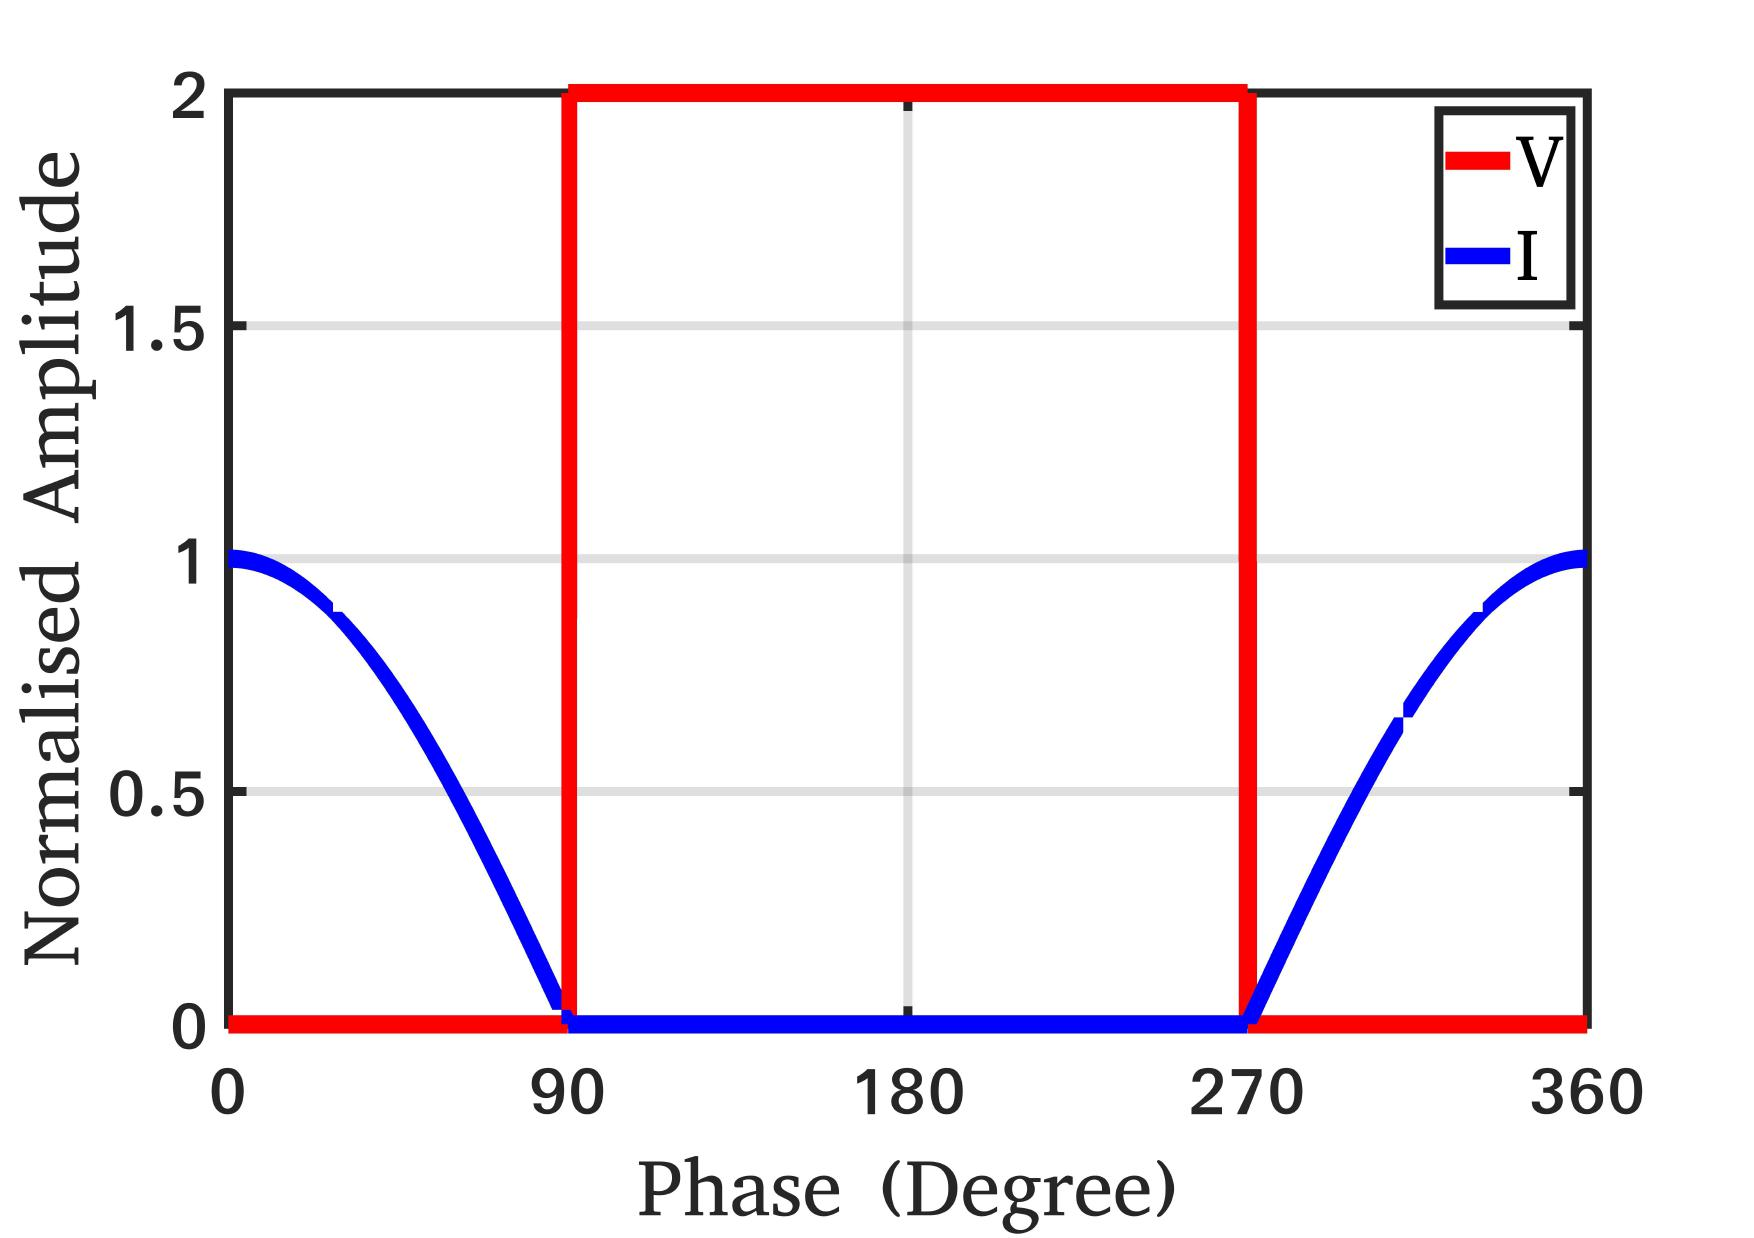
\includegraphics[width=1\textwidth]{Images/Intro/ClassF.pdf}
\caption{Ideal Class F}
\label{fig:ICF_wave_VI}
\end{subfigure}
\begin{subfigure}{0.24\textwidth}
\includegraphics[width=1\textwidth]{Images/Intro/CF_wave_VI_shaded.pdf}
\caption{Practical Class F}
\label{fig:CF_wave_VI}
\end{subfigure}
\caption{The class A/B/F drain  voltage/current (V/I) waveforms. \color{black}}
\label{fig:wave_VI}
\vspace{-0.25in}
\end{figure}
Generalized drain source-voltage ($V_{DS}$) containing all frequencies up to $3^{rd}$ harmonic \cite{Gen_Vds_eqn} is given by:
\begin{equation}
V_{DS}=\underbrace{1}_{\text{DC}}-\underbrace{\frac{2}{\sqrt{3}} \cos \theta}_{\text{$1^{st}$ harmonic}}+\underbrace{\frac{1}{3 \sqrt{3}} \cos 3 \theta}_{\text{$3^{rd}$ harmonic}}
\label{eqn_CF_V}
\end{equation}
The drain current ($I_{D}$), which is a half-sine wave, is given by
\begin{equation}
I_{D}=\underbrace{\frac{1}{\pi}}_{\text{DC}}+\underbrace{\frac{1}{2} \cos \theta}_{\text{$1^{st}$ harmonic}}+\underbrace{\frac{2}{3 \pi} \cos 2 \theta}_{\text{$2^{nd}$ harmonic}}-\underbrace{\frac{2}{15 \pi} \cos 4 \theta}_{\text{$4^{th}$ harmonic}}
\label{eqn_CCF_I}
\end{equation}
The load impedance at the  $1^{st}$, $2^{nd}$, and $3^{rd}$ harmonic are represented by $Z_{1f}=\frac{4}{\sqrt{3}}$, $Z_{2f}=0$, and $Z_{3f}=\infty$, respectively. As depicted in Fig. \ref{fig:CF_wave_VI},  one of the advantages of class F PAs is that its normalized peak drain voltage is two. Nonetheless, they suffer from limited operational bandwidth (typically 10\%) owing to the need for short and open circuit harmonic terminations. Thus, to realize wider bandwidth, the continuous class F (CCF) PA has been proposed \cite{CCF_reason}. In this paper, we present four different CCF passive output stages. 

\section{Continuous Class F}
\label{section:CCF}
\vspace{-0.05in}
Compared to class F, the CCF has an extra imaginary part at both the $1^{st}$/$2^{nd}$ harmonic of the voltage waveform. Thus, the generalized $V_{DS}$ for CCF is given by \cite{ECCF_Carrubba}:
\begin{equation}
V_{DS}=\underbrace{1}_{\text{DC}}-\underbrace{\frac{2}{\sqrt{3}} \cos \theta-\gamma \sin \theta}_{\text{$1^{st}$ harmonic}}+\underbrace{\frac{7 \gamma}{6 \sqrt{3}} \sin 2 \theta}_{\text{$2^{nd}$ harmonic}}+\underbrace{\frac{1}{3 \sqrt{3}} \cos 3 \theta}_{\text{$3^{rd}$ harmonic}}
\label{eqn_CCF_V}
\end{equation}
As in class F, $I_{D}$ is a half sinusoid (given in (\ref{eqn_CCF_I})). These equations indicate that $V_{DS}$/$I_{D}$ are chosen so that no power is dissipated at higher harmonics. Also, mathematically, the $\gamma$ in (\ref{eqn_CCF_V}) does not affect drain efficiency ($\eta_D$). But it affects the peak drain voltage, as depicted in Fig. \ref{fig:CCF_wave_VI}. In reality, however, $I_{D}$ depends on $V_{DS}$, degrading $\eta_D$ as $\gamma$ increases.


Fig. \ref{fig:CCF_wave_VI} implies that at $\gamma$ = 0, the waveform is like class F. For the $\gamma$ values between -1 and 1, $V_{DS}$ remains positive, enabling CCF PA to meet linearity requirements. However, CCF PAs suffer from large peak drain voltage which can be as high as 3.12 times the supply ($V_{DD}$) when $\gamma$ = -1 or 1. Using (\ref{eqn_CCF_V}) and (\ref{eqn_CCF_I}), the load impedance of CCF  are $Z_{1f}=\frac{4}{\sqrt{3}}+j 2 \gamma$, $Z_{2f}=0-j \frac{\pi}{2} \frac{7 \sqrt{3}}{6} \gamma$, and $Z_{3f}=\infty$ \cite{CCFDesign_ali}.


In CCF, $Z_{3f}$ remains open-circuited similar to class F. Meanwhile, $Z_{1f}$ and $Z_{2f}$ have a reactive part, unlike class F. From CCF load impedances and Fig. \ref{fig:CCF_SC}, it is perceived that if the reactive part of $Z_{1f}$ changes from inductive to capacitive, then the reactive part of $Z_{2f}$  needs to change from capacitive to inductive or vice-versa across the bandwidth to achieve CCF operation. In the next section, the design procedure for the proposed four output networks is meticulously presented. 


\begin{figure}[!t]
\captionsetup{font=footnotesize}
\centering
\begin{subfigure}{0.24\textwidth}
\centering
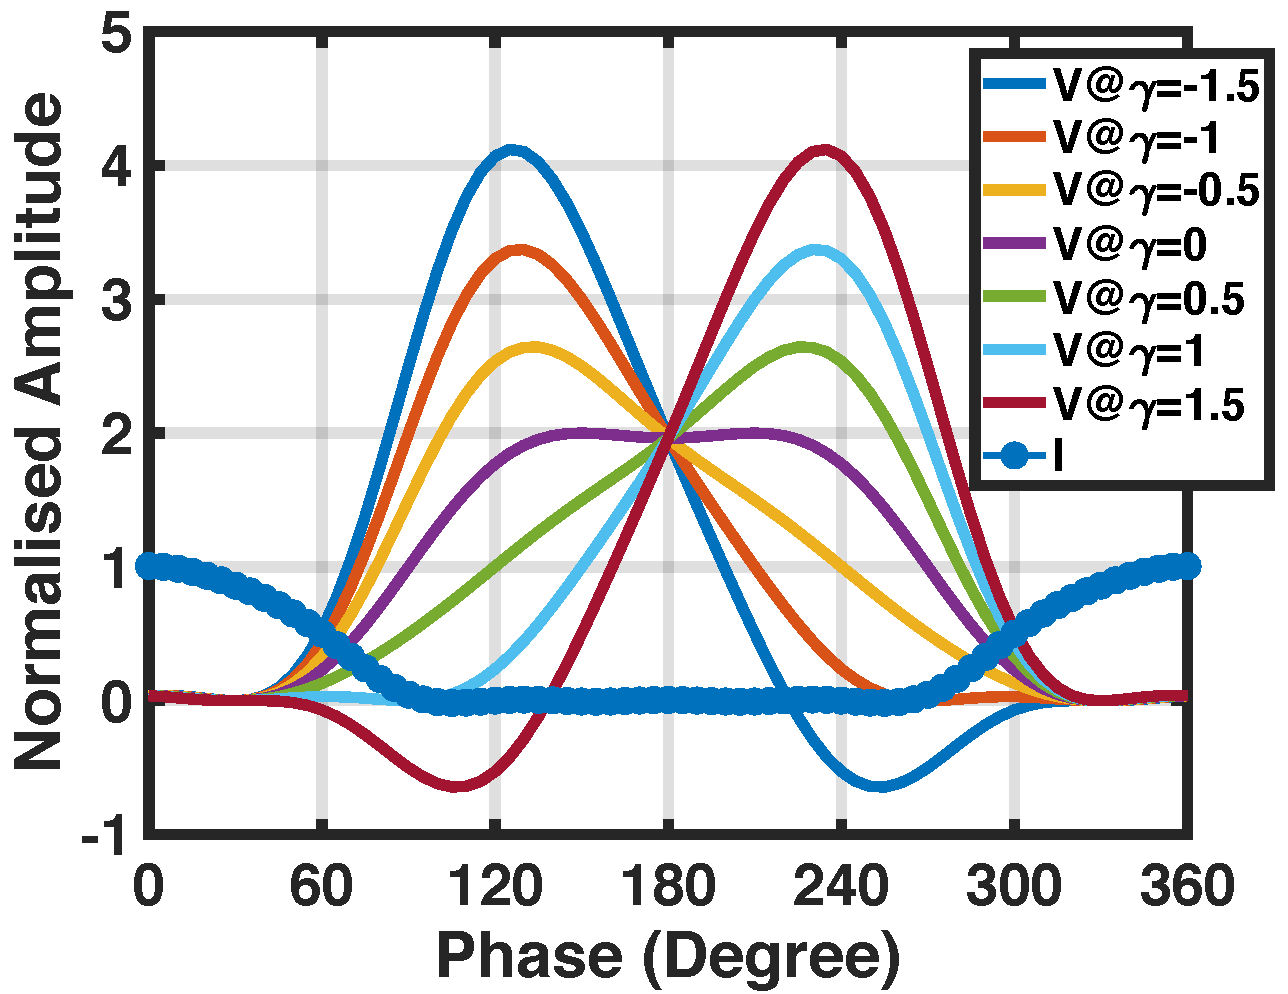
\includegraphics[width=1\textwidth]{Images/CCF/CCF_wave_VI.pdf}
\caption{}
\label{fig:CCF_wave_VI}
\end{subfigure}
\begin{subfigure}{0.24\textwidth}
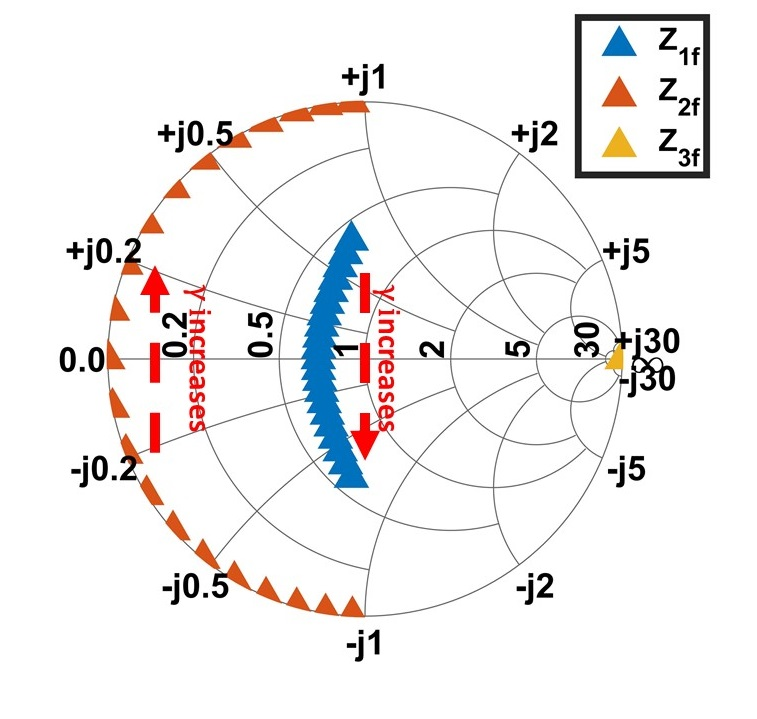
\includegraphics[width=1\textwidth]{Images/CCF/CCF_SC.jpg}
\caption{}
\label{fig:CCF_SC}
\end{subfigure}
\caption{(a) $V_{DS}$ and $I_D$ waveform for CCF with -1.5 $<$ $\gamma$ $<$ 1.5, and (b) Variation of $Z_{1f}$, $Z_{2f}$, $Z_{3f}$ for -1 $<$ $\gamma$ $<$ 1.}
\label{fig:CCF_VI_SC}
\vspace{-0.2in}
\end{figure}

 

\section{Design of Output Network for CCF}
\label{section:ON}
In this paper, the push-pull (differential) structure is chosen for the PA mainly because it decouples the odd harmonics ($1^{st}$/$3^{rd}$) from even harmonic ($2^{nd}$) impedance. Moreover, it suppresses supply/substrate noise, second-order nonlinearities and doubles the RF output power. 
In this work, the targeted peak RF power is 27dBm  while its operational bandwidth is 2.1--2.7GHz with $V_{DD}$ = 2.7V. To achieve this, a  fundamental differential impedance of 38.7$\Omega$ should be presented to the drains of the transistors across the 2.1--2.7GHz band, obtaining as follows:
\vspace{-0.05in}
\begin{equation}
\begin{aligned}
&V_{FUND-diff}=2\times V_{FUND-single}=2\times\frac{2}{\sqrt{3}} V_{DD}=6.24 \hspace{1mm}V\\
&R_{D-diff}=\frac{V_{FUND-diff}^{2}}{2\times\hspace{1mm} P_{OUT_{max}}}=38.7 \hspace{1mm} \Omega
\label{eqn_diff_imp}
\end{aligned}
\end{equation}
The requirements of the output network for CCF is exhibited in Tab. \ref{tab:Output_Network_Requirements}. The PA operates in class F mode at the center frequency $\omega_0$ (2.4GHz) with a short at $2\omega_0$ (4.8GHz) and an open at $3\omega_0$ (7.2GHz). But, for all other frequencies, the PA performs in the CCF mode. 

\setlength{\arrayrulewidth}{0.5mm}
\setlength{\tabcolsep}{2pt}
\renewcommand{\arraystretch}{1.5}
\begin{table}[!t]
\centering
\captionsetup{font=footnotesize}
\resizebox{\linewidth}{!}{%
\begin{tabular}{|c|c|c|c|}
\hline
\begin{tabular}[c]{@{}c@{}}\textbf{Class of} \\\textbf{Operation}\end{tabular} & \begin{tabular}[c]{@{}c@{}}\textbf{First Harmonic} \\($\omega$)\end{tabular} & \begin{tabular}[c]{@{}c@{}}\textbf{Second Harmonic} \\(2$\omega$)\end{tabular} & \begin{tabular}[c]{@{}c@{}}\textbf{Third Harmonic} \\(3$\omega$)\end{tabular} \\ \hline
\multirow{2}{*}{\textbf{\begin{tabular}[c]{@{}c@{}}Class F \\ (2.4GHz)\end{tabular}}} & $\Re(Z_D)$ = 38.7$\Omega$ & $\Re(Z_D)$= 0$\Omega$ & \multirow{2}{*}{\begin{tabular}[c]{@{}c@{}}$|Z_D|\approx$ 1000$\Omega$\end{tabular}} \\ \cline{2-3}
 & $\Im(Z_D)$ = 0$\Omega$ & $\Im(Z_D)$ = 0$\Omega$ &  \\ \hline
\multirow{2}{*}{\textbf{\begin{tabular}[c]{@{}c@{}}\\CCF \\ (2.1--2.7GHz)\end{tabular}}} & $\Re(Z_D)$ = 38.7$\Omega$ & $\Re(Z_D)$ = 0$\Omega$ & \multirow{2}{*}{\begin{tabular}[c]{@{}c@{}}\\$|Z_D|\approx$ 1000$\Omega$ \end{tabular}} \\ \cline{2-3}
 & \begin{tabular}[c]{@{}c@{}}$\Im(Z_D)$ $\rightarrow$ + to -\\ OR\\ $\Im(Z_D)$ $\rightarrow$ - to +\end{tabular} & \begin{tabular}[c]{@{}c@{}} $\Im(Z_D)$ $\rightarrow$ - to +\\ OR\\ $\Im(Z_D)$ $\rightarrow$ + to -\end{tabular} &  \\ \hline
\end{tabular}%
 }
\caption{Output network specifications.}
\label{tab:Output_Network_Requirements}
\vspace{-0.25in}
\end{table}

The proposed four different  output networks, comprising passive lumped components are illustrated in Fig. \ref{fig:Design_A_FC} and \ref{fig:Design_B_C_D}a/b/c. 
All the designs consist of a balun and a load capacitance ($C_L$). The balun converts the balanced (differential) signal to its single-ended companion, whereas $C_L$ adjusts $3^{rd}$ harmonic impedance. The power transistor's drain-source capacitance (assume $C_{DS}=1.87$pF) is absorbed into the output network to reduce its impact on the PA performance. The balun is modeled using an ideal transformer, consisting of magnetizing inductance ($L_m$), leakage inductance ($L_k$), primary inductance ($L_P$), and coupling coefficient ($km$) \cite{Transformer_model}. 

\subsection{Design A (no RF choke \& with $L_2C_2$)}
Design A consists of a $2^{nd}$ harmonic trap ($L_2C_2$), which provides short at $2\omega_0$. The $V_{DD}$ is supplied through the balun's center tap, and $L_{BND}$ is used to model bond-wire inductance ($\approx$1nH). Analysis of the schematics is performed in differential-/common-mode scenarios by utilizing the equivalent circuits depicted in Fig. \ref{fig:Design_A}b/c, respectively, to calculate the unknown parameters: transformer's coupling factor ($km$) and turn ratio ($N$) along with  $L_P$, $C_2$, $L_2$, and $C_L$. Fig. \ref{fig:Design_A_Diff} shows that the drain impedance ($Z_D$) is given by
\vspace{-0.05in}
\begin{equation}
	Z_D=\left(\frac{1}{\frac{j\omega C_{DS}}{2}}+\frac{1}{Z_{SB}}\right)^{-1}=38.7 \hspace{1mm} \Omega
	\label{eqn:ZD}
\end{equation}

\begin{figure}[!t]
\captionsetup{font=footnotesize}
\centering
\begin{subfigure}{0.5\textwidth}
\centering
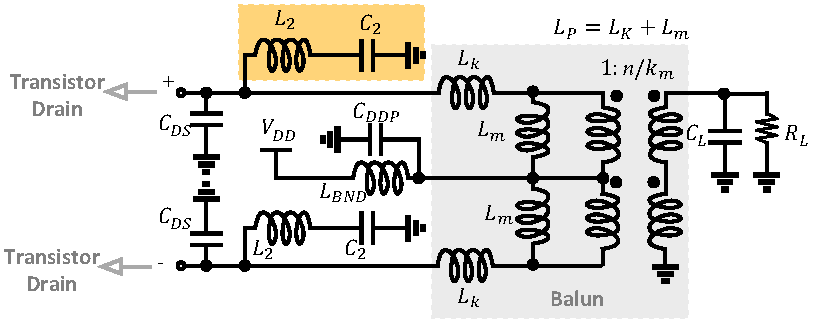
\includegraphics[width=1\textwidth]{Images/Design/Design_A_FC.pdf}
\caption{}
\label{fig:Design_A_FC}
\end{subfigure}
\begin{subfigure}[b]{0.35\textwidth}
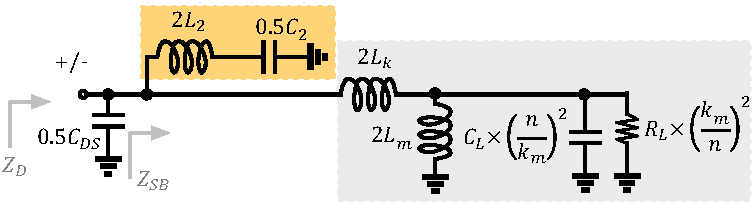
\includegraphics[width=1\textwidth]{Images/Design/Design_A_Diff.pdf}
\caption{}
\label{fig:Design_A_Diff}
\end{subfigure}
\begin{subfigure}[b]{0.35\textwidth}
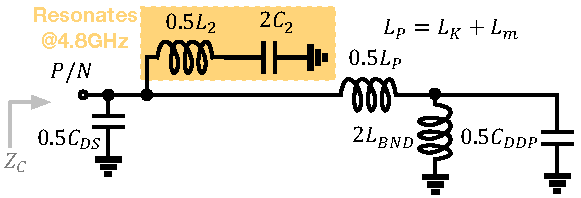
\includegraphics[width=1\textwidth]{Images/Design/Design_A_Com.pdf}
\caption{}
\label{fig:Design_A_Com}
\end{subfigure}
\caption{(a) Design A (Balun, $L_2C_2$ and $C_L$), (b) differential-mode, and (c) common-mode equivalent circuit }
\label{fig:Design_A}
\vspace{-0.2in}
\end{figure}

The value of $Z_{SB}$ (impedance of $L_2C_2$ and balun given by (\ref{eqn:Design_A_ZSB})) that will provide $Z_D$ of 38.7$\Omega$ can be calculated from (\ref{eqn:ZD}) and the value is $\Re(Z_{SB})(\omega_0) =  29.8\Omega$ and $\Im(Z_{SB})(\omega_0) = 16.6\Omega$.
\vspace{-0.05in}
\begin{equation}
\begin{aligned}
    &Z_{SB}=\left(\frac{1}{Z_B}+\frac{1}{Z_S}\right)^{-1}
    \hspace{1mm}\text{where}, Z_S=2j\omega  L_2+\frac{1}{\frac{j \omega C_2}{2}}, \\
    &Z_B=\left(\frac{1}{R_P}+\frac{1}{2j \omega  L_m}+j \omega C_P\right)^{-1}+2j \omega  L_k,\\ &R_P=R_L\left(\frac{km}{n}\right)^2,C_P=C_L\left(\frac{n}{km}\right)^2
\label{eqn:Design_A_ZSB}
\end{aligned}
\end{equation}

It is evident from (7) that $C_{DS}$ should resonate with $\Im(Z_{SB})$ to attain high drain impedance at $3\omega_0$. This implies $\Im(Z_{SB})(3\omega_0) = 24.96\Omega$. Ideally, $\Re(Z_{SB})(3\omega_0)$ should be 0 to achieve high $3^{rd}$ harmonic impedance. However, Fig. \ref{fig:Design_A_Rn_var_1H} depicts that having a larger $\Re(Z_{SB)}(3\omega_0)$ contributes to a constant $P_{OUT}$ across the operational bandwidth by flattering the real part at the fundamental. Another benefit is that it has a  more linear reactive part at the fundamental, which is essential in CCF operation.
However, this leads to a lower $3^{rd}$ harmonic impedance, as showcased in Fig. \ref{fig:Design_A_Zn_3H}. This also emphasizes  the significance of $C_L$. Thus, to achieve 1000$\Omega$ at $3^{rd}$ harmonic,  $\Re(Z_{SB})(3\omega_0) = 0.5\Omega$, which is obtained from Fig. \ref{fig:Design_A_Zn_3H}. Fig. \ref{fig:Design_A_Com} proves that $L_2$ should have a series resonance with $C_2$ to get short at 2$\omega_0$.

\vspace{-0.05in}
\begin{equation}
    L_2=\frac{1}{4\times\omega_0^2\times C_2}%=0.73 \hspace{1mm} nH
    \label{eqn:Design_A_2H}
\end{equation}

\begin{figure}[!t]
\captionsetup{font=footnotesize}
\centering
\begin{subfigure}{0.24\textwidth}
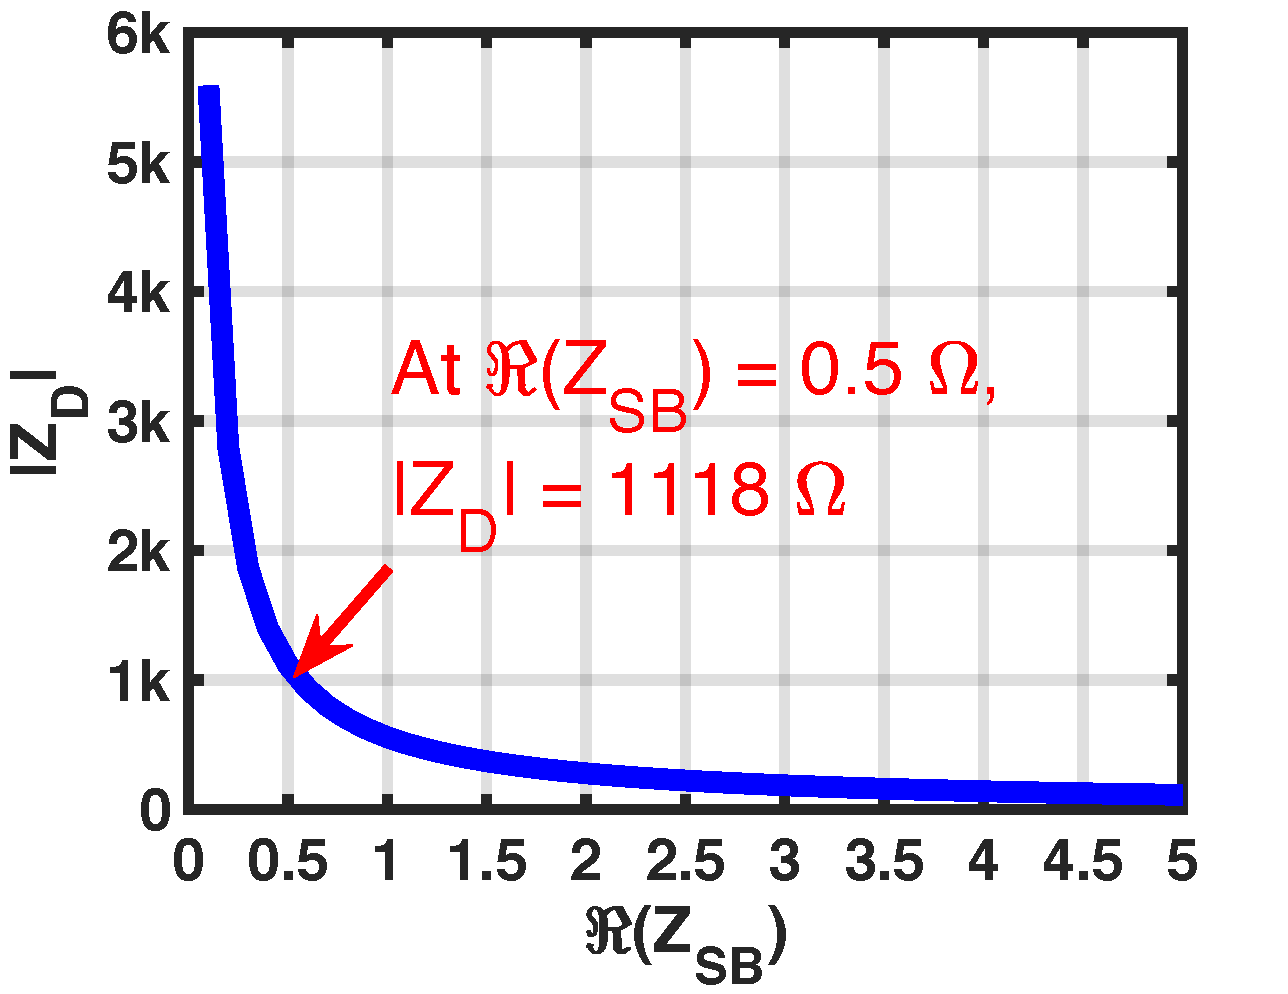
\includegraphics[width=1\textwidth]{Images/Design/Design_A_Zn_3H.pdf}
\caption{}
\label{fig:Design_A_Zn_3H}
\end{subfigure}
\begin{subfigure}{0.24\textwidth}
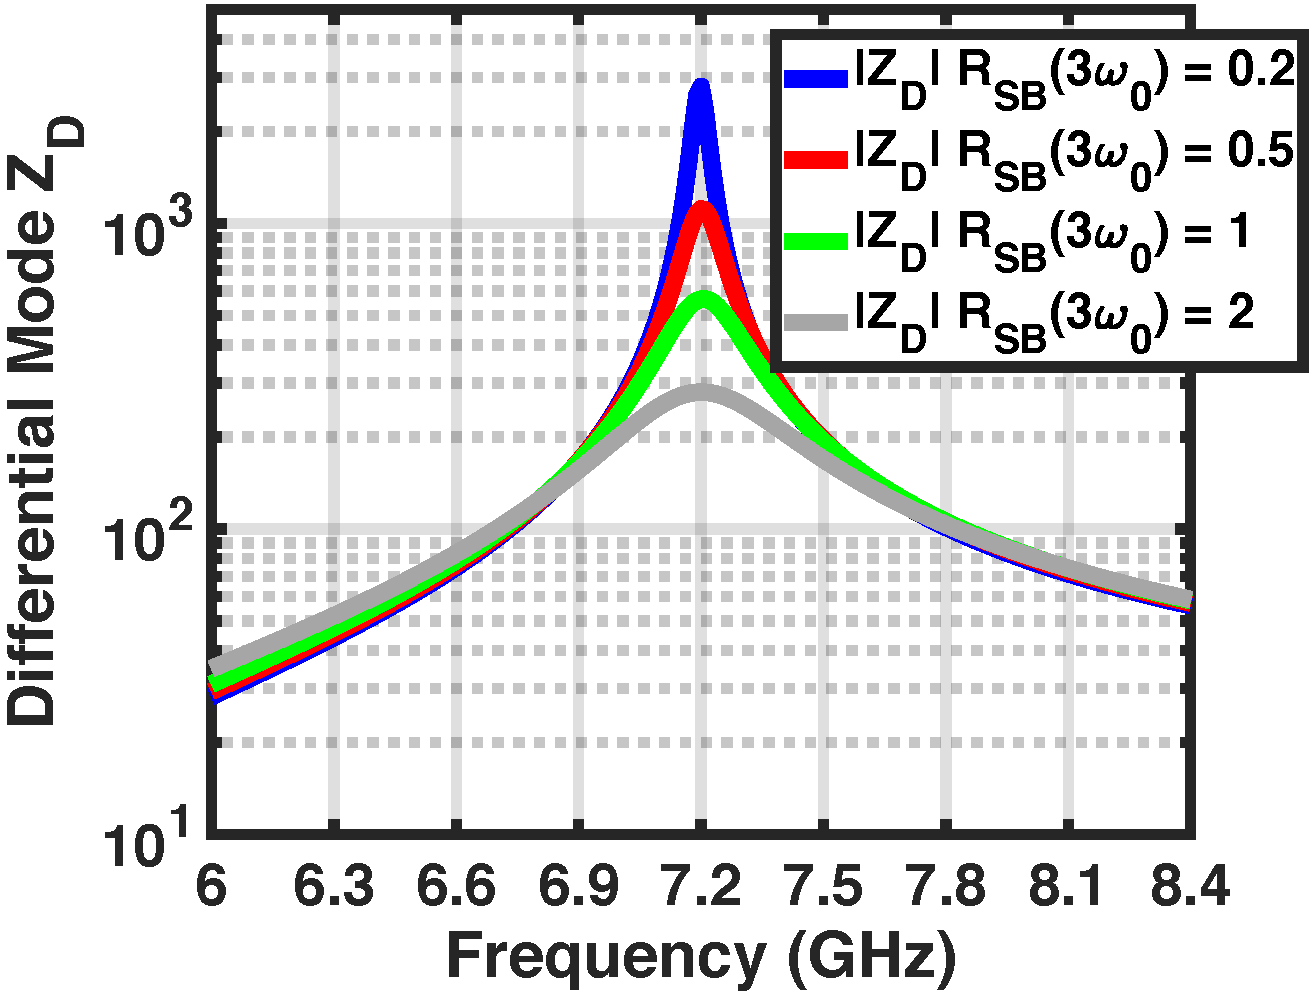
\includegraphics[width=1\textwidth]{Images/Design/Design_A_Rn_var_3H.pdf}
\caption{}
\label{fig:Design_A_Rn_var_3H}
\end{subfigure}
\begin{subfigure}{0.5\textwidth}
\centering
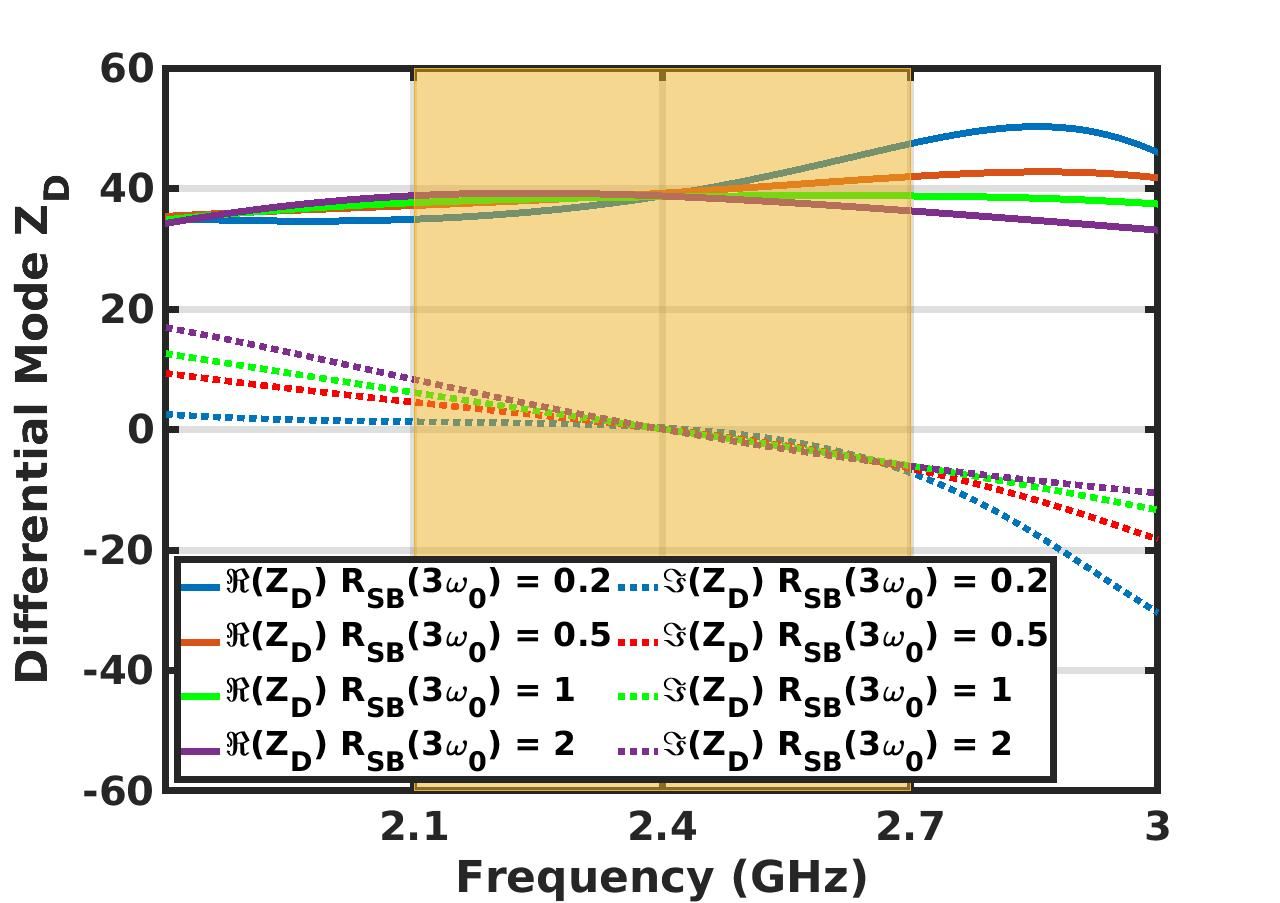
\includegraphics[width=0.55\textwidth]{Images/Design/Design_A_Rn_var_1H.jpg}
\caption{}
\label{fig:Design_A_Rn_var_1H}
\end{subfigure}
\caption{(a) Magnitude of $Z_{D}$ vs $\Re(Z_{SB})$ at $3\omega_0$, (b) Magnitude of $Z_D$ at $3^{rd}$ harmonic for various $R_{SB}(3\omega_0)$, and (c) $Z_D$ at fundamental for various $R_{SB}(3\omega_0)$.}
\label{fig:Design_A_Rn_var}
\vspace{-0.2in}
\end{figure}

The five unknowns in the circuit: $km$, $N$, $L_P$, $C_2$, and $C_L$ can be calculated by assuming one of them and using four equations ($\Re(Z_{SB})(\omega_0) =  29.8 \Omega$, $\Im(Z_{SB})(\omega_0) = 16.6\Omega$, $\Re(Z_{SB})(3\omega_0) = 0.5\Omega$ and  $\Im(Z_{SB})(3\omega_0) = 24.96\Omega$). In this paper, $km =$ 0.8 is assumed and the remaining unknowns ($N =$ 1.34, $L_P =$ 2.2nH, $C_L =$ 0.9pF, $C_2 =$ 1.5pF, $L_2 =$ 0.73nH are calculated. The $km$ can be varied to get different sets of results in which $L_P$ is minimal and thereby making it layout friendly.


\subsection{Design B (no RF choke \& no $L_2C_2$)}

\begin{figure}[!t]
\captionsetup{font=footnotesize}
\centering
\begin{subfigure}{0.2\textwidth}
\centering
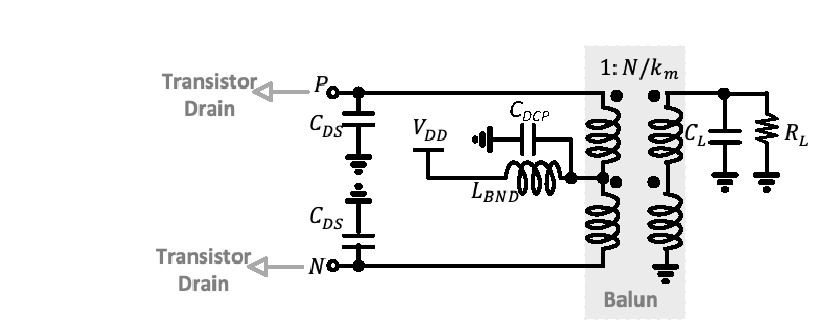
\includegraphics[width=1\textwidth]{Images/Design/Design_B_FC.pdf}
\caption{}
\label{fig:Design_B_FC}
\end{subfigure}
\begin{subfigure}{0.26\textwidth}
\centering
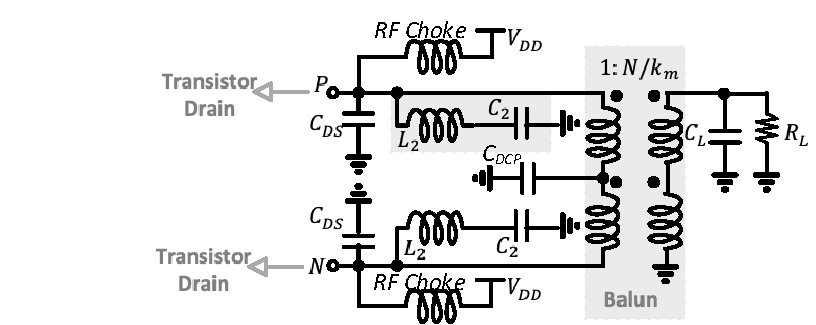
\includegraphics[width=1\textwidth]{Images/Design/Design_C_FC.pdf}
\caption{}
\label{fig:Design_C_FC}
\end{subfigure}
\centering
\begin{subfigure}{0.24\textwidth}
\centering
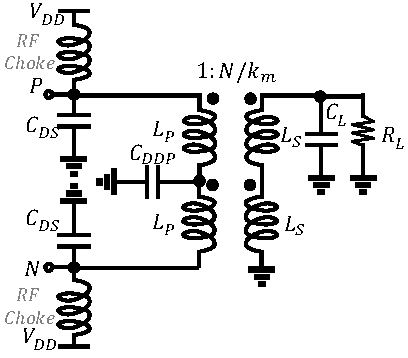
\includegraphics[width=1\textwidth]{Images/Design/Design_D_FC.pdf}
\caption{}
\label{fig:Design_D_FC}
\end{subfigure}
\caption{(a) Design B (Balun and $C_L$), (b) Design C (Balun, RF Choke, $L_2C_2$ \& $C_L$), and (c) Design D (Balun, RF Choke \& $C_L$).}
\label{fig:Design_B_C_D}
\vspace{-0.25in}
\end{figure}

In this design (Fig. \ref{fig:Design_B_FC}), $L_2C_2$ is removed, reducing the number of unknowns. Like the previous case, differential mode analysis yields four equations, and there are four unknowns, thus leading to a single set of values for $km =$ 0.72, $N =$ 0.9, $L_P =$ 0.63nH, $C_L =$ 3.96pF, unlike design A. $C_{DDP}$ is tuned to provide a short at $2\omega_0$ such that $C_{DDP}$ resonates with $L_P$, $L_{BND}$, and $C_{DS}$, which is obtained from the common-mode analysis. Moreover, $C_{DDP}$ provides RF ground and blocks DC.

\subsection{Design C (with RF choke \& with $L_2C_2$)}
In this design (Fig. \ref{fig:Design_C_FC}), $V_{DD}$ is supplied through RF choke, unlike the previous designs. RF chokes are assumed to have a fixed value of 5nH. The differential mode analysis yields four equations similar to design A. Assuming $km =$ 0.8, the other unknowns are calculated as $N =$ 1.14, $L_P =$ 2.23nH, $C_L =$ 1.10pF, $C_2 =$ 1.37pF.
Like design A, $C_2$ should resonate out with $L_2$ to get short at $2\omega_0$. Thus, $L_2 =$ 0.8nH. 

\subsection{Design D (with RF choke \& no $L_2C_2$)}
 Unlike design C, $L_2C_2$ is removed in this design (Fig. \ref{fig:Design_D_FC}). Also, RF choke should be calculated, assuming $C_{DS}$ resonates with it at $\omega_0$ (RF Choke = 2.35nH).
The differential mode analysis yields four equations and the four unknowns ($N =$ 0.84, $L_P =$ 0.86nH, $C_L =$ 3.95pF, $km =$ 0.77) can be calculated.
$C_{DDP}$ can be tuned to provide a short at $2\omega_0$.

\begin{figure}[!t]
	\captionsetup{font=footnotesize}
	\centering
	\begin{subfigure}{0.5\textwidth}
		\centering
		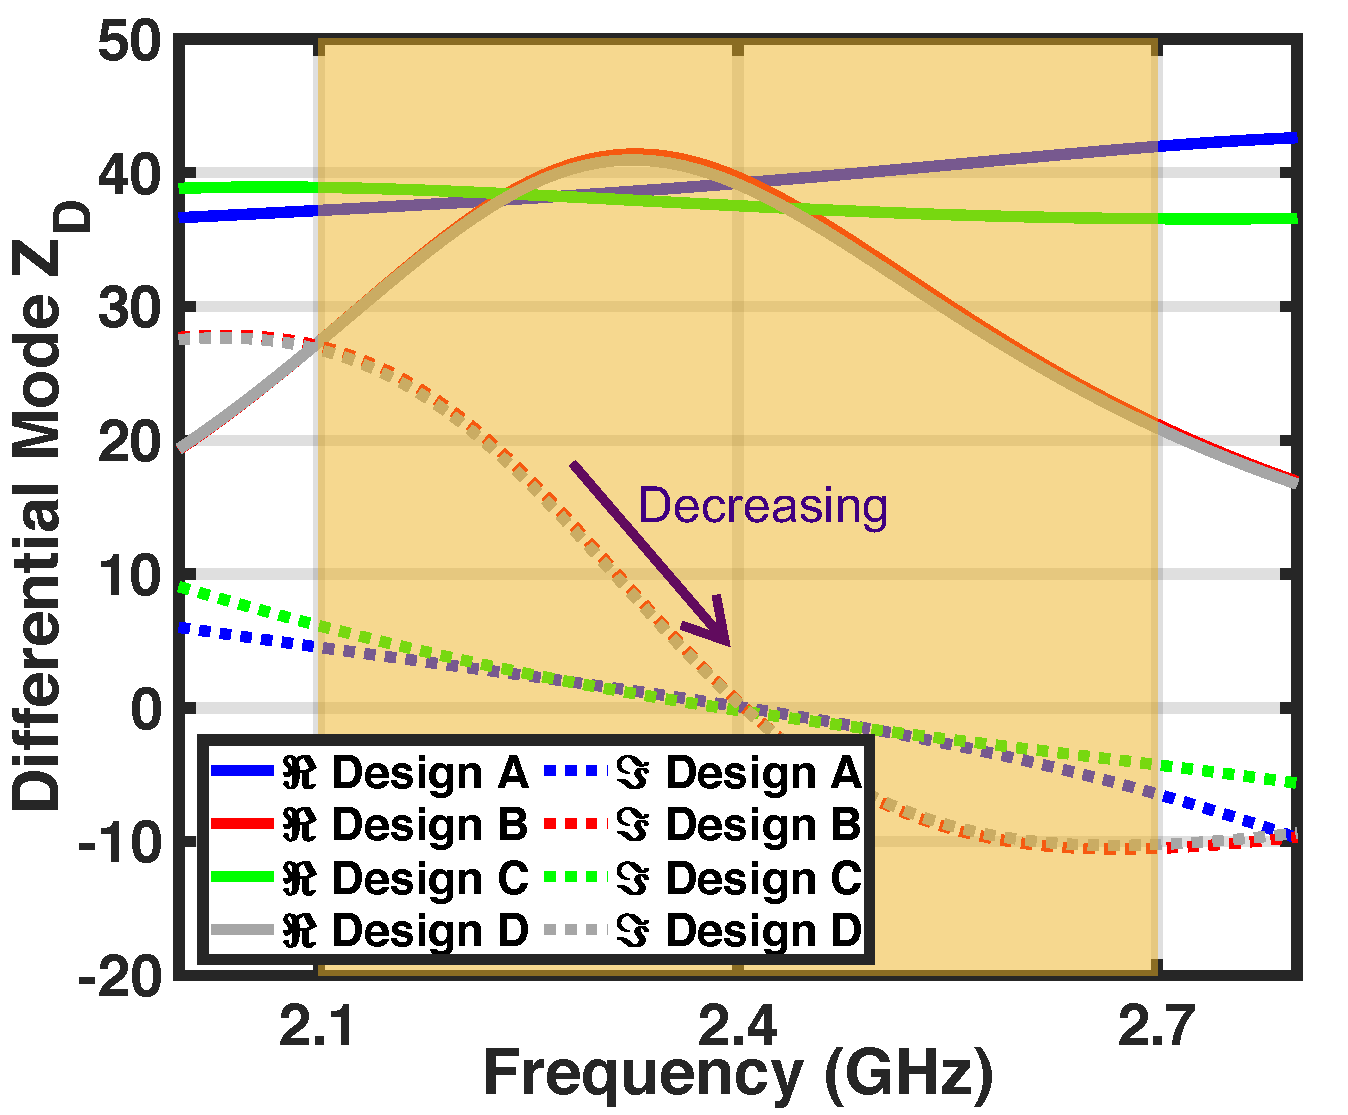
\includegraphics[width=0.55\textwidth]{Images/Output_Network_Comp/Comp_1H.pdf}
		\caption{}
		\label{fig:Comp_1H}
	\end{subfigure}
	\begin{subfigure}{0.24\textwidth}
		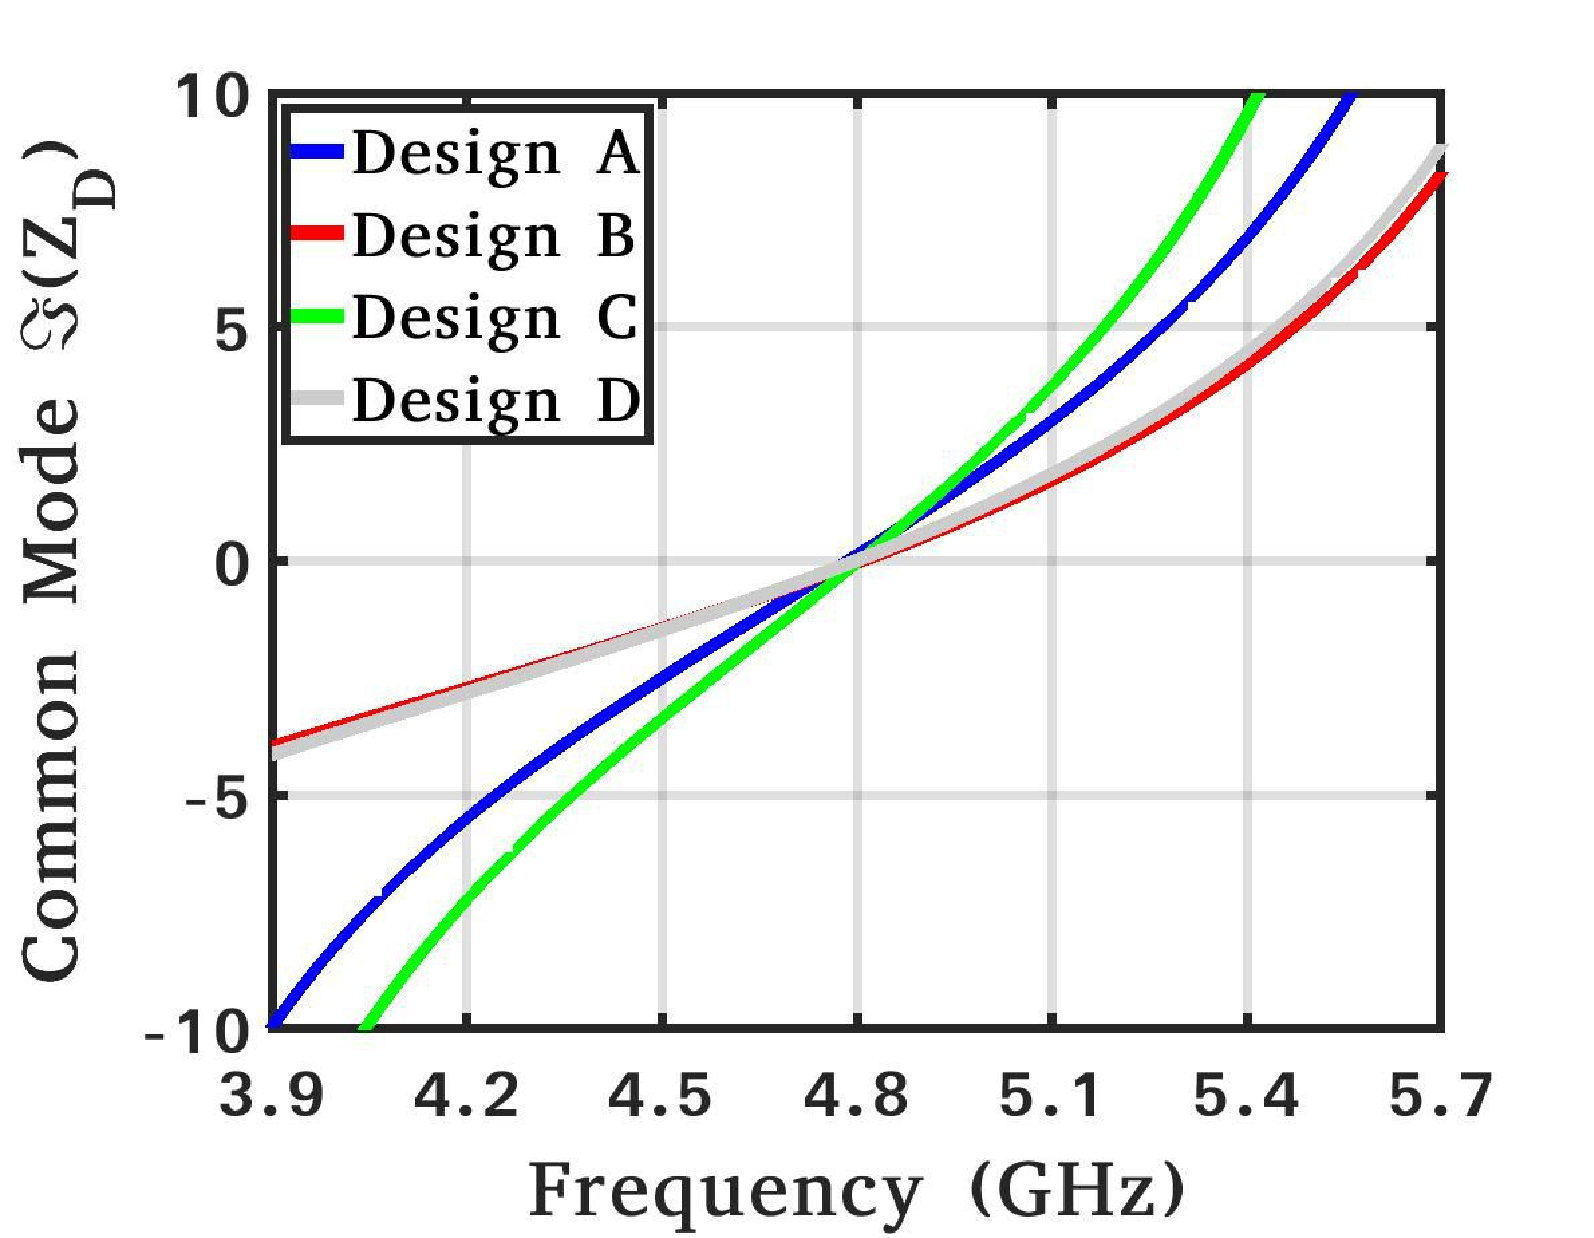
\includegraphics[width=1\textwidth]{Images/Output_Network_Comp/Comp_2H_imag.pdf}
		\caption{}
		\label{fig:Comp_2H_imag}
	\end{subfigure}
	\begin{subfigure}{0.24\textwidth}
		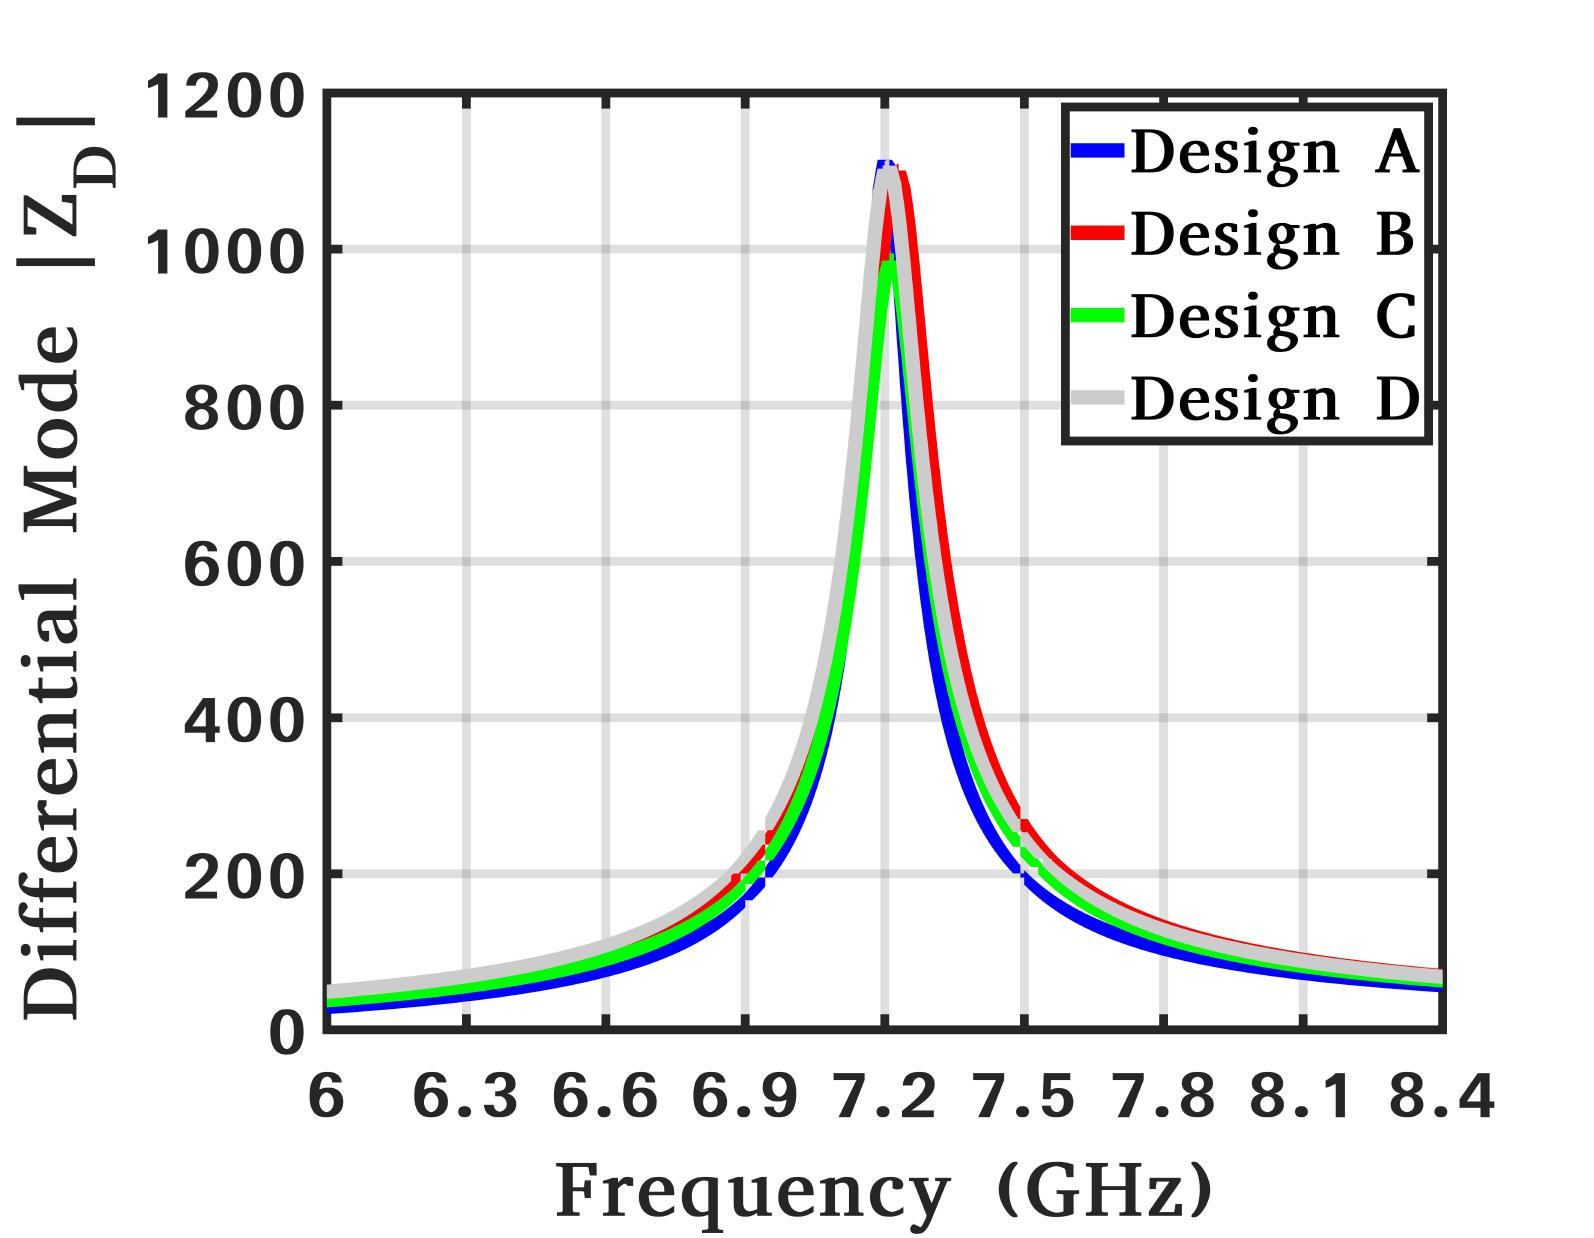
\includegraphics[width=1\textwidth]{Images/Output_Network_Comp/Comp_3H_Mag.pdf}
		\caption{}
		\label{fig:Comp_3H_Mag}
	\end{subfigure}
	\caption{(a) Impedance ($Z_D$) at $1^{st}$ harmonic, (b) Reactive part of $Z_D$ ($\Im(Z_D)$) at $2^{nd}$ harmonic, and (c) Magnitude of $Z_D$ ($|Z_D|$) at $3^{rd}$ harmonic.}
	\label{fig:Comp_1H_2H_3H}
	\vspace{-0.1in}
\end{figure}

\section{Results}
\label{section:Results}

Fig. \ref{fig:Comp_1H_2H_3H} shows that all the four designs satisfy the main CCF requirement, which is a decreasing trend of the reactive part at the fundamental and increasing trend of the reactive part at $2^{nd}$ harmonic. As illustrated in Fig. \ref{fig:Comp_1H}, the real part in the desired frequency band is flatter for design A/C, which leads to constant $P_{OUT}$, unlike design B/D. Moreover, to fully accomplish CCF operation, the series $L_2C_2$, which resonates at the $2^{nd}$ harmonic, acts as a capacitor at the desired band. The designs B/D have a higher reactive part at the fundamental than other designs, contributing to a larger $\gamma$ value and, thus, higher peak drain voltage (Fig. \ref{fig:CCF_wave_VI}). Fig. \ref{fig:Comp_1H_2H_3H}b/c show that all designs have a similar response at $2^{nd}$/$3^{rd}$ harmonics. Nevertheless, design A generates a more constant $P_{\text{OUT}}$ in the band of interest and has minimal passive components. 

To validate the proposed output passive stage,  design A is laid out in an LP 40nm CMOS process (Fig. \ref{fig:ON_X1}) with a 600$\mu m$ balun. In this context, $km=$ 0.69 is selected to achieve a layout friendly $L_P$/$L_S$. Hence, all design parameters are re-calculated. Subsequently, design A is simulated in three different forms. A lossless network, a lossy condition (with a quality factor of 7,  13, and 100 for inductors, balun, and capacitors, respectively), and the proposed layout. The ADS (Momentum) simulation results are depicted in Fig. \ref{fig:Comp_Pout_DE}, which indicates, there are relatively good agreements between the lossy and the proposed layout with a 68\% passive efficiency at 2.4GHz. Moreover, using an ideal push-pull PA, the proposed design achieves peak RF output power/drain efficiency of more than 25dBm/62\%, respectively, over the desired frequency band. 

\begin{figure}[!t]
\centering
\captionsetup{font=footnotesize}
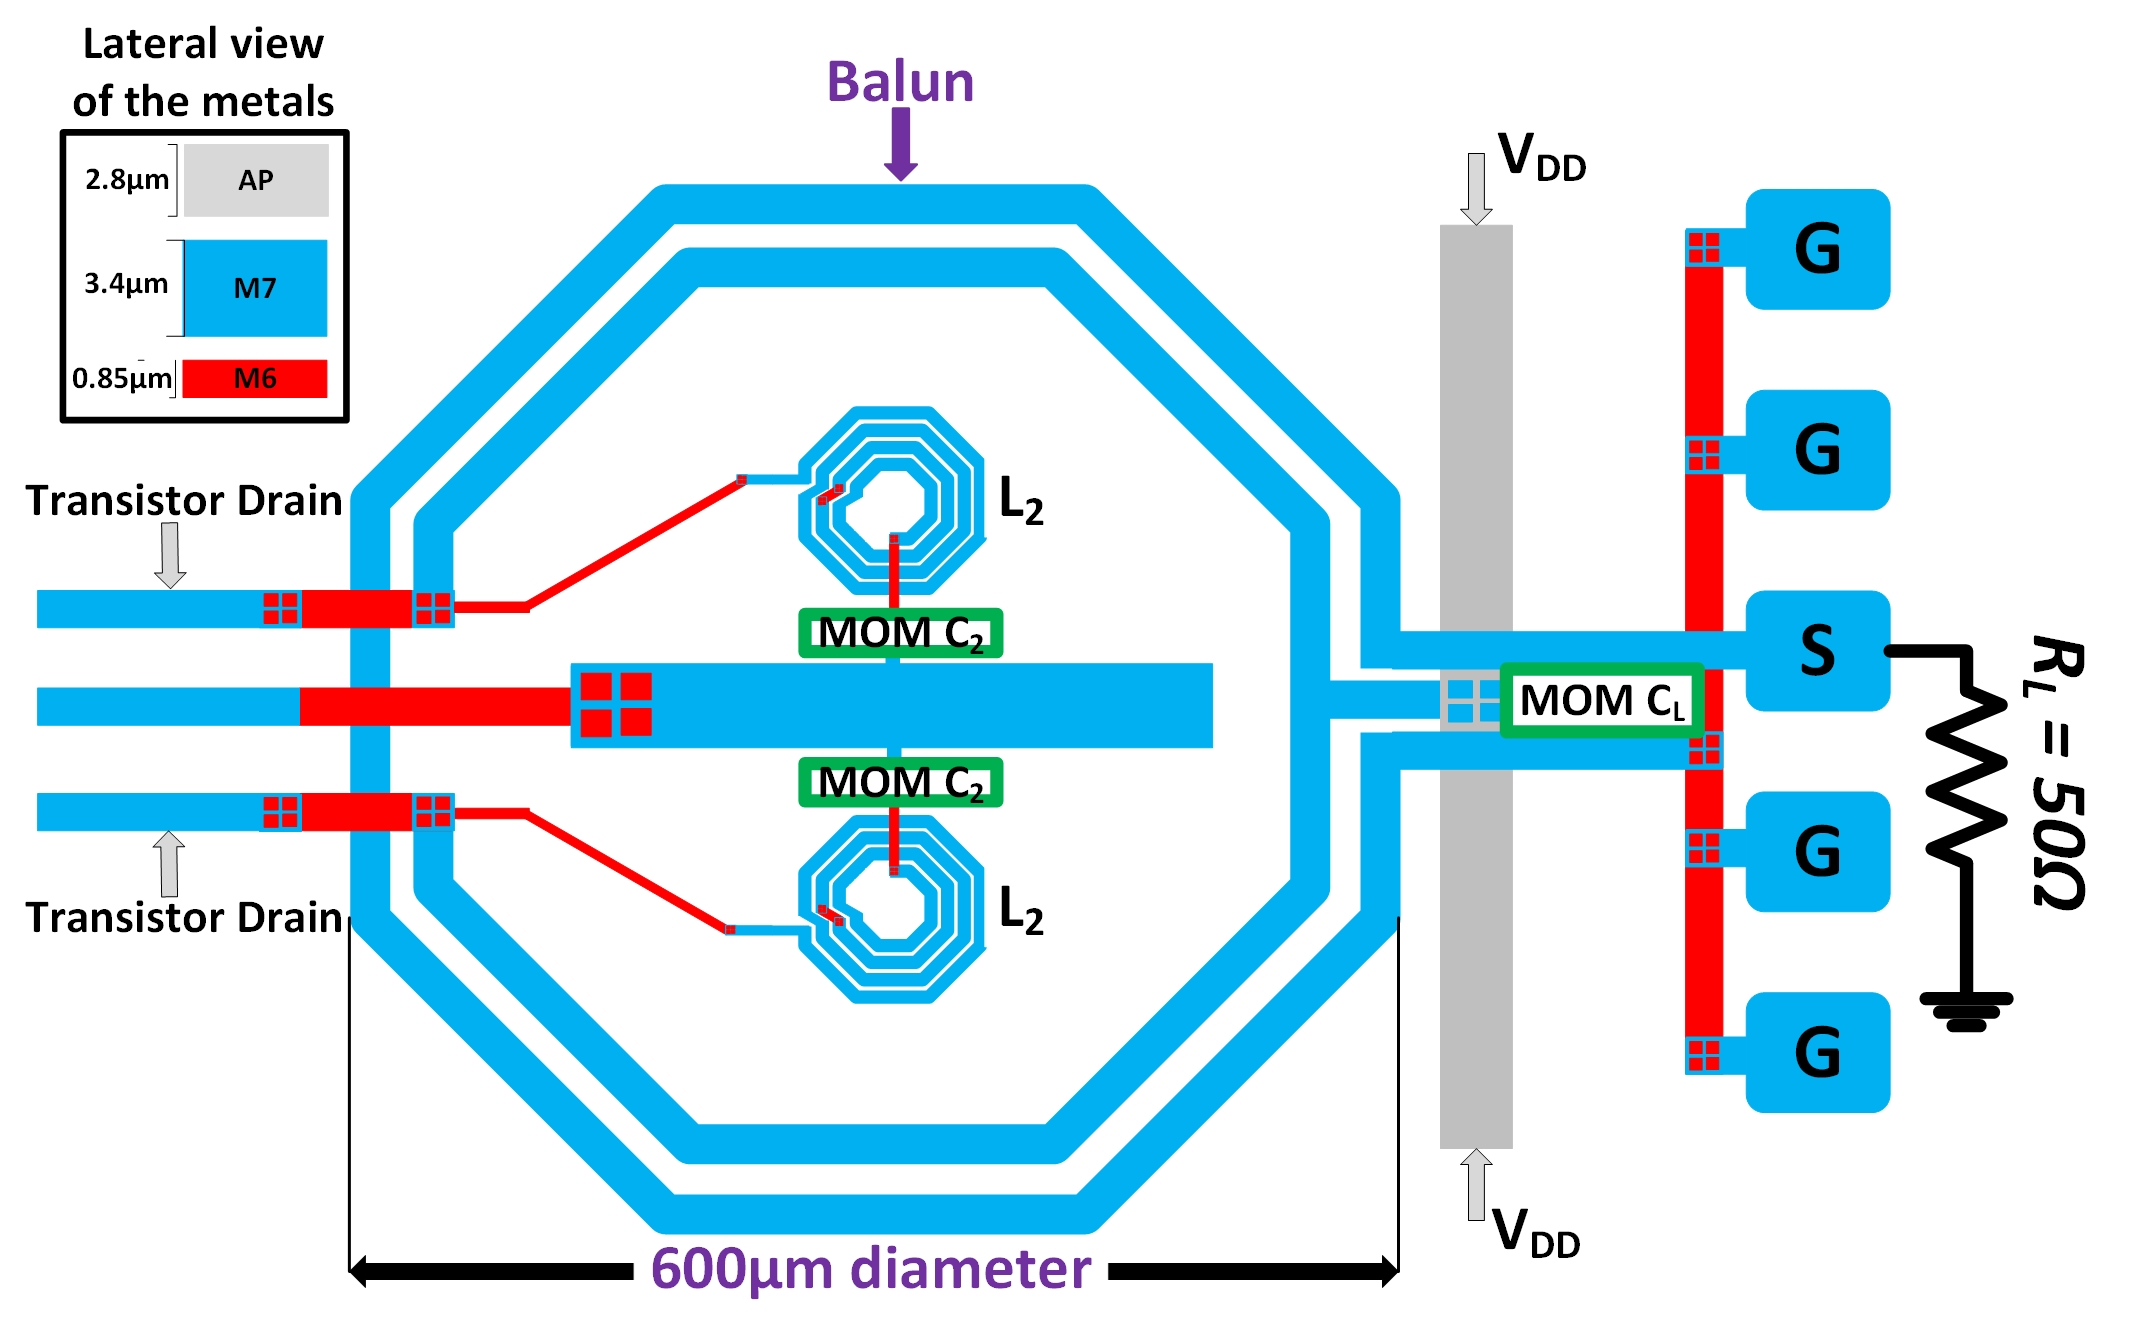
\includegraphics[width=1\linewidth]{Images/Output_Network_Comp/Balun_V2.jpg}
\caption{Layout of the design A (balun, $L_2C_2$ and $C_L$).}
\label{fig:ON_X1}
\vspace{-0.1in}
\end{figure}

\begin{figure}[!t]
\captionsetup{font=footnotesize}
\centering
\begin{subfigure}{0.24\textwidth}
\centering
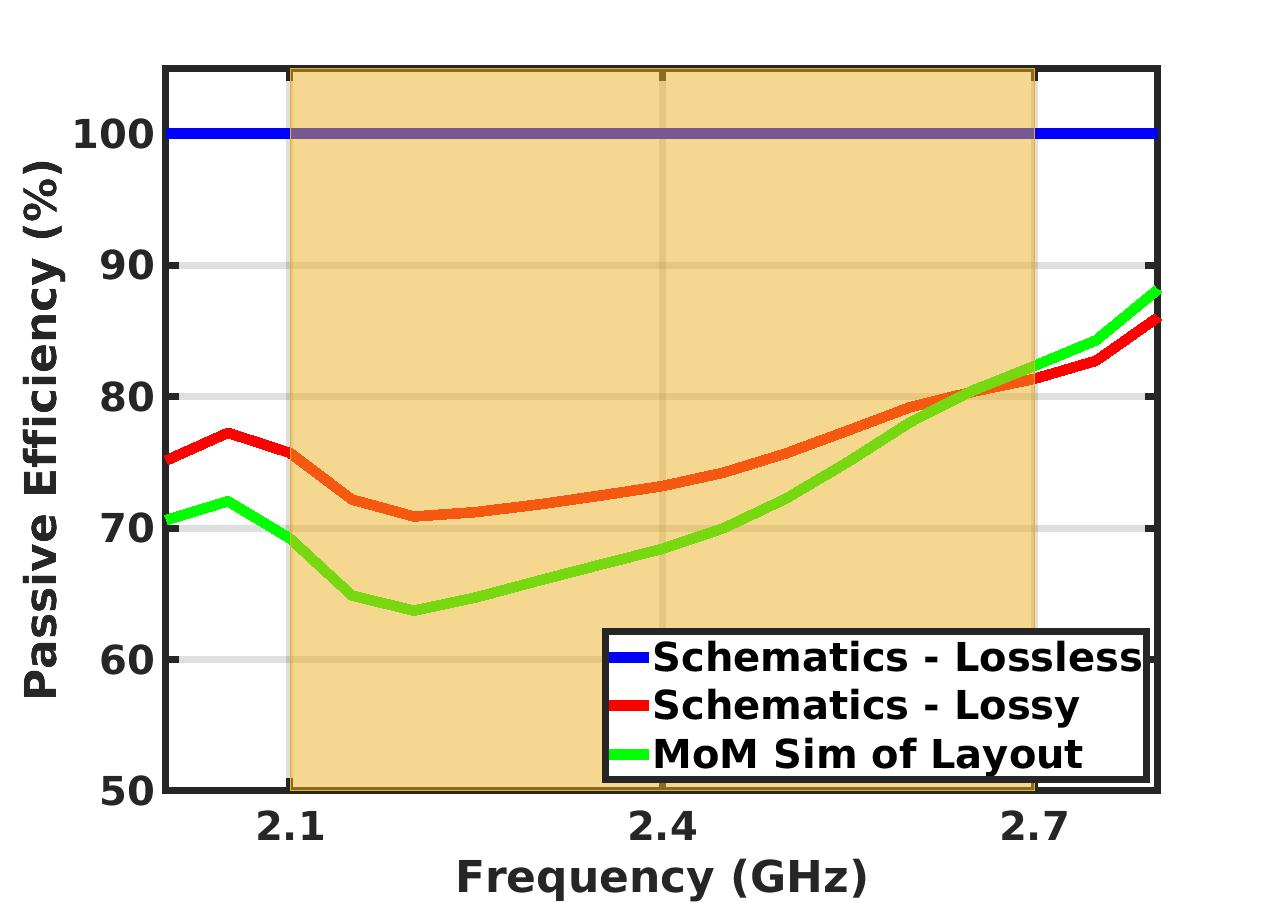
\includegraphics[width=1\textwidth]{Images/Output_Network_Comp/Comp_PasEff_loss_layout_km0p69.jpg}
\caption{}
\label{fig:Comp_PasEff_loss_layout_km0p69}
\end{subfigure}
\begin{subfigure}{0.24\textwidth}
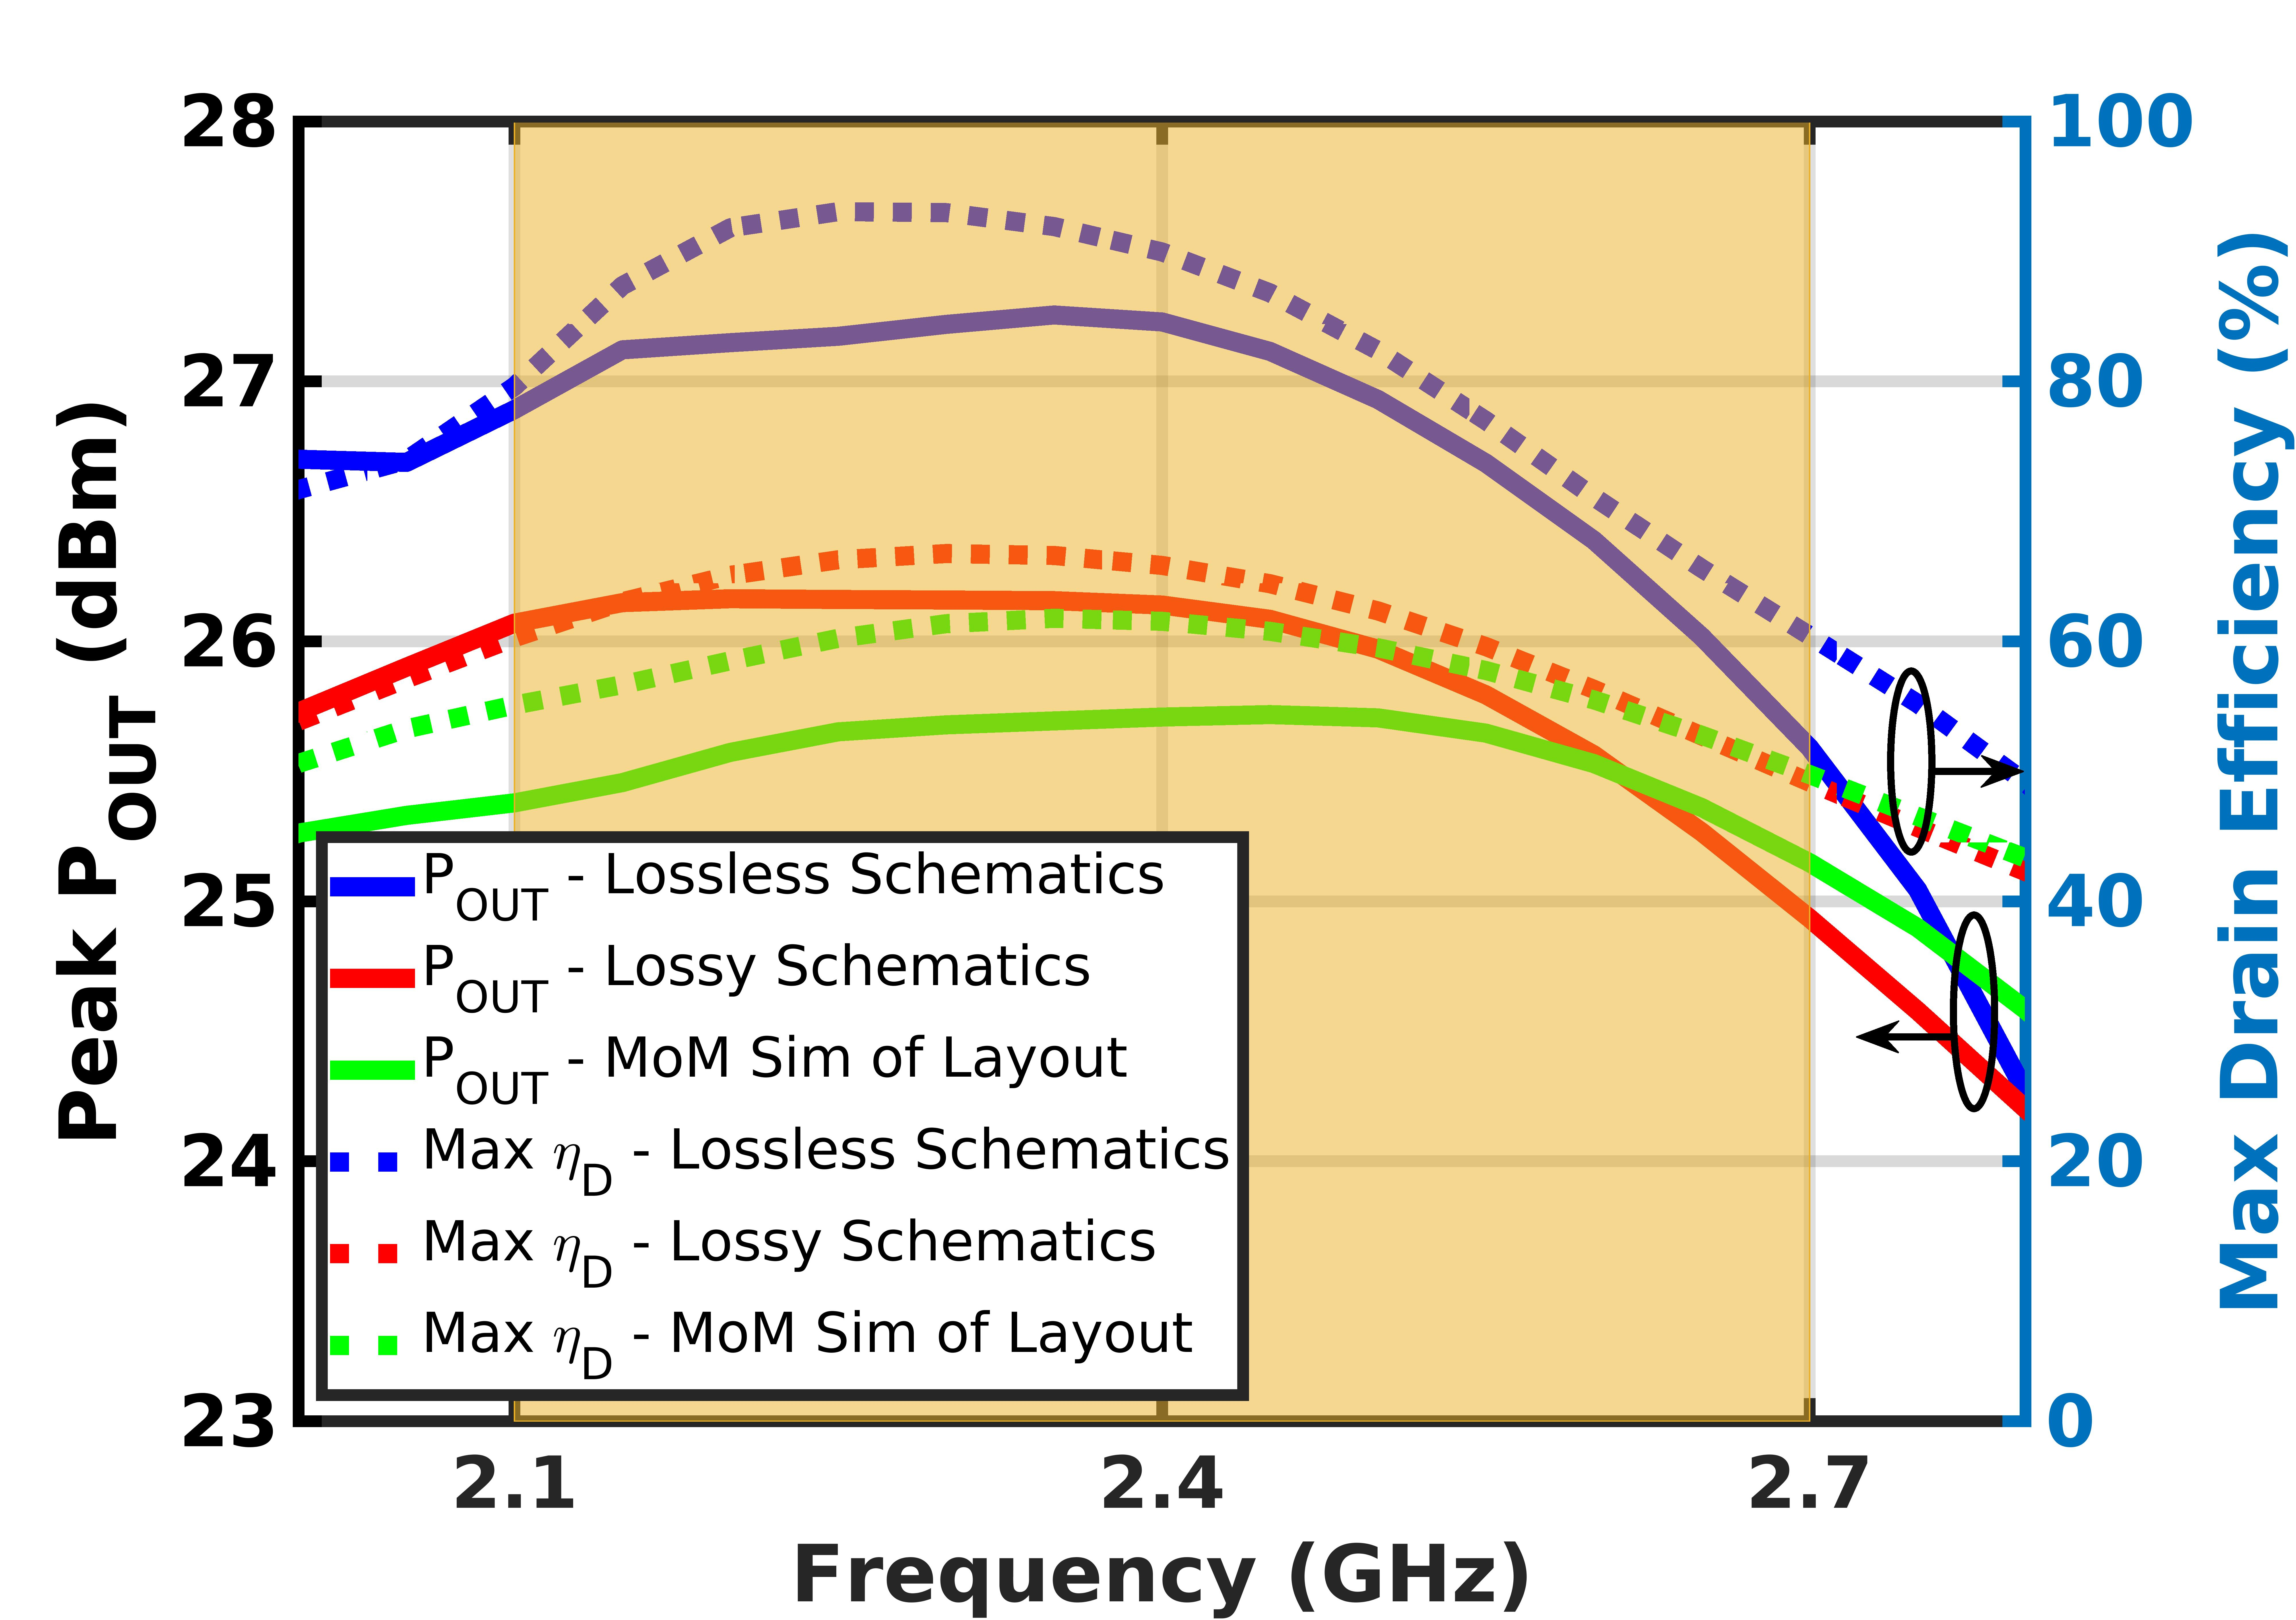
\includegraphics[width=1\textwidth]{Images/Output_Network_Comp/Comp_Pout_DE_loss_layout_km0p69.jpg}
\caption{}
\label{fig:Comp_Pout_DE_loss_layout_km0p69}
\end{subfigure}
\caption{(a) Passive efficiency, and (b) Maximum $P_{OUT}$ and drain efficiency versus frequency band.}
\label{fig:Comp_Pout_DE}
\vspace{-0.25in}
\end{figure}

\section{Conclusion}
\label{section:Conclusion}
In this paper, the primary advantage of CCF PAs over its class F companion is presented. It details the critical requirement of the CCF PA output network, which is if the $1^{st}$ harmonic reactive part decreases, its $2^{nd}$ harmonic reactive part increases. Furthermore, the design procedure of various output networks for the 2.1 -- 2.7GHz band is presented, and the proposed passive output stages are synthesized.  Consequently, design A, with no RF choke and a 2$^{nd}$ harmonic trap, is chosen due to its relatively constant output RF power in the desired frequency band with minimal on-chip passive components. This design is laid out in a 40nm CMOS while achieving a 68\% passive efficiency at 2.4GHz.

\bibliographystyle{IEEEtran}
\bibliography{ISCASvABS.bib}

\end{document}


